%\documentclass{article}
%\usepackage{graphicx,subfigure}
%\begin{document}

\begin{figure}[!h]
  \centering
  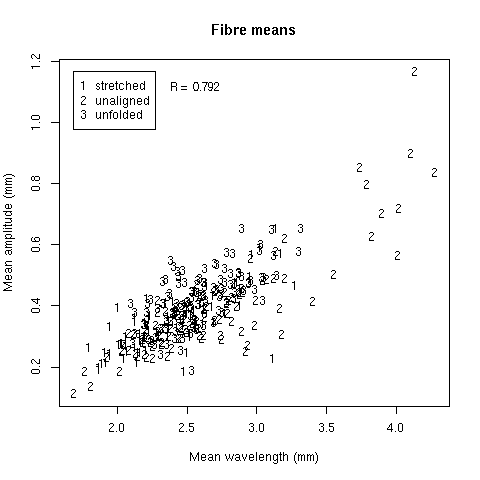
\includegraphics[width=1.0\textwidth]{figsffibremeans.png}
%   fibremeanswa.png is original 
  \caption{Correlation between fibre means for Wavelength and Amplitude with CrimpType identified for each fibre. Means are averages over 30 waves per fibre.}
  \label{fig:sffibremeans}
\end{figure}

%\end{document}

